\documentclass{standalone}

\usepackage{tikz}
\usetikzlibrary{calc}
\usetikzlibrary{decorations.markings}


\begin{document}
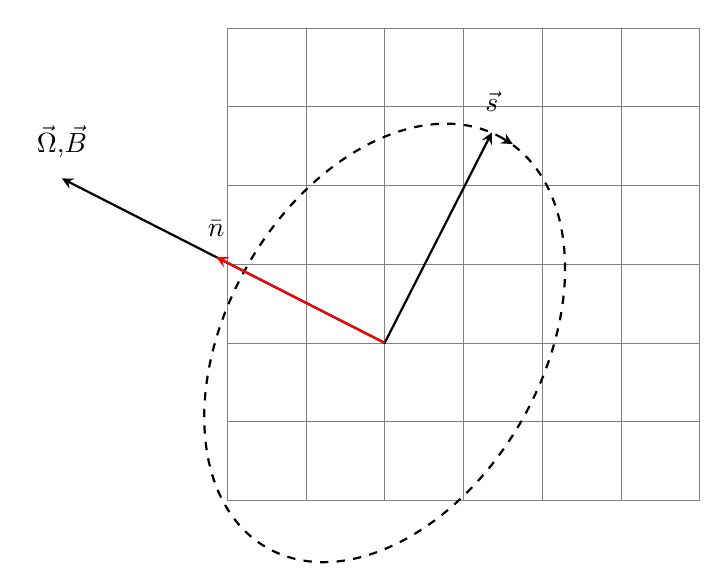
\begin{tikzpicture}[>=stealth, line width=.8pt]
	\draw[help lines] (-2,-2) grid (4,4);
	\node (c) at (0,0) {.};
	\node[blue,label=above:{$\vec\Omega$,$\vec B$}] (B) at ($(c)+(153:4.6cm)$) {};
	\node[red,label=above:$\bar n$] (nbar) at ($(c)+(153:2.4cm)$) {};
	\node[label=above:$\vec s$] (sp) at ($(c)+(63:3cm)$) {};
	\draw[rotate=60, dashed,
		decoration={markings, mark=at position 1 with {\arrow{<}}},
		postaction={decorate}]  circle [x radius=3cm, y radius=2cm];
	\draw[->] (c.center) -- (sp.center);
	\draw[->] (c.center) -- (B.center);
	\draw[->, red] (c.center) -- (nbar.center);
\end{tikzpicture}
\end{document}